\chapter{跨期价差}
跨期价差也叫作时间价差(time spread),它涉及卖出一个期权,同时买入一个更远期的期权,两个期权的行权价相同。从广义上说,跨期价差是一个水平价差。使用跨期价差的中性哲学是,时间对近期期权价值的侵蚀速度要比对远期期权快。如果是这样的话,在短期期权到期时,价差就会变宽,交易者能得到盈利。交易者还可以用看涨期权来构建一个更为激进的牛市跨期价差。

1 月下旬有下面的价格:XYZ:50,XYZ 4 月 50 看涨期权(3 个月期权):5,XYZ 7 月 50 看涨期权(6 个月期权):8,XYZ 10 月 50 看涨期权(9 个月期权):10。

假定在 3 个月后 4 月合约到期时,XYZ 的价格仍然是 50,没有变化。这样的话,3 个月的看涨期权应当价值 5 点,6 个月的看涨期权应当价值 8 点。

4 月 50 与 7 月 50 之间的价格差现在扩大到 5 点。因为这个价差最初的支出是 3 点,价格差的扩大就产生了 2 点盈利。

要产生盈利,标的股票在近期合约到期日时并不一定需要刚好等于近期期权行权价。事实上,在高于和低于该行权价的范围内,都可以产生一些盈利。这类头寸的风险是股票会大幅下跌或上涨。在这样的情况下,两个期权之间的价格差就会缩小,交易者就会亏钱。\textbf{由于同一行权价的两个期权的价格差不可能缩小到低于零。因此,这个价差的风险就限制在最初建立这个价差时的支出金额内,再加上手续费。}

\section{中性跨期价差}
进行跨期价差交易的交易者,要么对股票价格中性,要么对股票强烈看多。我们首先介绍一下中性的情况。一个跨期价差,如果在建立时标的股票价格刚好等于或者接近所用期权的行权价,那么它就是一个中性的价差。这个策略家感兴趣的是卖出时间,而不是预测标的股票的方向。如果在近期期权到期时股票相对没有变化,这个中性价差就可以盈利。在一个中性价差里,交易者一开始就应当计划在近期期权到期时将这个价差平仓。

\begin{figure}[h]
    \centering
    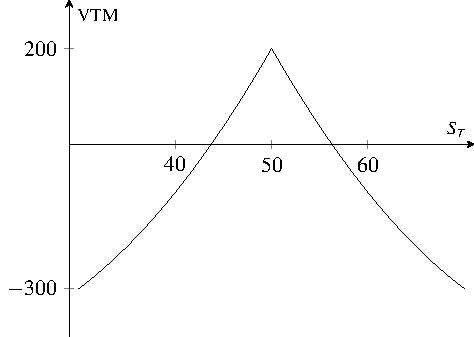
\includegraphics[width=0.7\textwidth]{IMG/Calendar spread at near-term expiration.pdf}
    \label{fig:calendar spreads}
\end{figure}

一般而言,建立这样一个价差的最好时间是在近期期权到期之前的 8-12 个星期。如果这样做,交易者就能赚到近期期权相对较长期期权最大比率的因时减值。
\subsection{波动率的影响}
期权的隐含波动率(也就是标的股票的实际波动率)对这个跨期价差会有影响。随着波动率的增长,这个价差的跨度会增大;随着波动率的萎缩,这个价差的跨度会减小。知道这一点很重要。事实上,\textbf{买入跨期价差是一种反波动率策略:交易者希望标的物的价格保持不变。}有时当标的股票的波动率很大时,跨期价差看上去特别有吸引力。不过,这种看法可能是存在误区的。有两个原因:首先,因为这个股票是高波动率的,它有很大可能会运动到盈利区域之外;其次,如果股票确实稳定下来,在一个接近行权价的范围内交易,那么这个价差就会失去它的价值,因为它失去了波动性。这笔损失会大于从因时减值中得到的收益。
\section{后续行动}
理想情况下,这个价差交易者会希望股票价格在近期看涨期权到期时低于行权价。如果是这样,他可以只花一笔手续费就将这个价差平仓,也就是卖出先前买入的看涨期权所需要的手续费。而如果这两个看涨期权在到期时都是实值的,他就不得不付两笔手续费来将价差平仓。

如果标的股票很早就发生了向下穿破,价差交易者就有若干选择。他可以立刻将价差平仓,接受这个头寸的小额亏损。另一个选择是不去管它,直到近期期权到期,希望到时股票会有部分反弹,从而可以从价差的多头腿中得到部分弥补。这种继续持有头寸的做法往往比立刻平仓要好。因为买回先前卖出的看涨期权,可能需要很大比例的支出。另一种风险更大的下行防御行动是在股票开始剧烈下跌时卖出先前买入的看涨期权。这样做的话,价差交易者可以立刻从价差的多头腿中得到部分弥补,然后期望股价保持弱势,从而价差的空头腿可以无价值到期。要采取这个行动,交易者就必须要有足够的质押物为最终的裸看涨期权提供保证金,抵押物的金额常常超过最初建立价差时的支出。此外,如果标的股票价格反转,涨到或超过行权价,价差的空头腿就是裸头寸,会产生严重的亏损。这样的后续行动所承担的风险违背了价差最初的中性宗旨,因此是应当避免的。在这三种下行防御行动里,最容易和最保守的行动是什么都不做,让卖出的看涨期权无价值到期,然后希望标的股票回升。如果采取这个办法,风险就保持在最初建立价差时的支出金额内,有的时候股票的反弹还能给买入的看涨期权带来大笔盈利。虽然这样的反弹并不经常出现,但价差交易者并不需要付出什么。只要有这样的反弹出现,交易者就能得到好处。

事实上,即使这个价差没有亏损很多,价差交易者也可以使用这类行动来做某些细微修正。如果标的股票在近期到期时小幅低于行权价,卖出的期权就会无价值到期,价差交易者手里就会留下买入的期权头寸。他可以立刻将多头腿卖出,得到一笔小额盈利或亏损。不过,合理的策略常常是卖出一部分多头腿,以收回部分或全部初始投资,然后再继续持有剩余头寸。如果股票上涨,剩余的多头腿会显著增值。虽然这类行动偏离了这个时间价差的真正本质,但它并没有带来太大的风险。

标的股票价格很早就向上突破的处理方法与向下突破时相同。什么都不做常常是最好的行动。如果标的股票在价差建立后不久就上涨,价差的跨度就会缩小一些,但不会缩小很多。因为在上涨过程中,两个期权都会有时间价值。如果价差交易者急急忙忙地将头寸平仓,他就需要为两个相当贵的期权支付手续费。他最好再等一等,价格有很大可能性会反转。事实上,即使是在近期到期时,买入的期权正常情况下也会有一些时间价值,不会出现最大损失。在抵御上行运动方面可以采取的一个高风险的行动,是在技术性突破时买回卖出的看涨期权,并继续持有买入的看涨期权。如果突破失败并且价格下跌,这就可能带来灾难性的后果,实际损失可能远远超过最初的支出。因此,这样的行动对于中性策略家来说,是极端激进和没有逻辑的。

如果没有出现突破,随着时间的流逝,这个价差交易者一般会得到未兑现的盈利。如果出现这种情况,他就应当为自己设立某些心理停止点(stop-out points)。例如,如果距到期日只剩下两个星期,而标的股票价格相当接近行权价,那这个价差中的潜在盈利就会更大一些。但如果股价开始远离行权价,价差交易者就应当准备迅速平仓。这样的话,他不仅给盈利的积累留下了足够的空间,同时也采取了措施来保护已经产生的盈利。这与卖出比率者所采取的行动有些相像。在时间变得越来越少的时候,卖出比率者会缩小他的行动点的范围。

\section{牛市跨期价差}
有些更为激进的投资者偏向于使用不那么中性、更为看多的跨期价差。在一个牛市跨期价差中,交易者也是卖出近期的看涨期权和买入较远期的看涨期权,但标的股票价格会比这些看涨期权的行权价低一定幅度。这类头寸的吸引力在于其较低的投资额和较大的潜在盈利。当然,这里也是有风险的。

资者可以用下面的方式建立一个牛市跨期价差:
\begin{itemize}
    \item XYZ 普通股股票:45
    \item 按 1 卖出 XYZ 4 月 50 看涨期权
    \item 按 1.50 买入 XYZ 7 月 50 看涨期权
\end{itemize}
这个投资者希望发生两件事。第一件事是,他希望近期期权无价值到期。这就是用虚值期权来建立牛市跨期价差的原因:为了增加卖出的看涨期权无价值到期的机会。如果这种情况发生,投资者就能以等于最初的支出的净成本来得到较远期的看涨期权。

这个投资者希望发生的第二件事是:在 7 月 50 看涨期权到期时,股票的价格必须上涨。在这个示例里,即使 XYZ 在 4 月-7 月之间只上涨到 52,7 月 50 看涨期权就可以卖到至少 2 点。这是一个显著的收益百分比,因为这个看涨期权的成本已经被降低到 0.50 点。因此,假设短期看涨期权已经无价值到期,而标的股票价格在较远期看涨期权到期前高于其行权价,那这个牛市跨期价差就有大量的盈利。

投资者所希望的这两个条件同时发生的概率有多大呢?卖出的看涨期权会无价值到期的机会相当大,因为它是个短期看涨期权,并且股票价格一开始就低于行权价。如果股票下跌,或者甚至略为上升(靠近但不是超过行权价),第一个条件就会满足。最大的问题一般在第二个条件上,也就是标的股票价格在较远的到期日之前超过行权价。发生这种情况的机会一般很小,但如果发生了,就能得到很大的收益。因此,\textbf{这个策略提供了小概率获取大笔盈利的机会}。事实上,一笔大额的盈利可以很容易地抵消掉许多笔亏损,因为这些亏损都是小额的。当然,这个亏损代表了 100\% 的最初投资,因此投资者不可以将他所有的钱都投在牛市跨期价差里。

如果价差交易者建立这个价差时遵循了下面的标准,这个策略就是一种合理的投机方式。
\begin{enumerate}
    \item 选择一个波动率足够大,能在给定的时间内运动到行权价之上的股票。用股票价格远低于行权价的低波动股票来建立牛市跨期价差,就会显得非常“便宜”。不过如果要求股价必须在几个月里发生像 20\% 这样大的运动,那就不值得在一个低波动的股票上建立牛市跨期价差。
    \item 不要使用高于当前市价 1 档行权价的期权。例如,如果 XYZ 是 26,就应该使用 30 的行权价,而不要使用 35 的行权价。因为股价上涨到 30 的机会比上涨到 35 的机会要多出好几倍。
    \item 不要在牛市跨期价差上投入大比例的可用交易资金。
\end{enumerate}
\section{后续行动}
如果标的股票在近期看涨期权到期之前上涨,该牛市价差的交易者\textbf{千万不能}考虑将这个价差“分腿”,或考虑以亏损价买回先前卖出的看涨期权并希望买入的看涨期权能继续盈利。这两个行动都会将最初的小额有限亏损转变成灾难性的亏损。因为这个策略依靠这样的事实:所有的亏损都是小额的,少数大额盈利能够抵消这些小额亏损。因此,投资者不应当做任何会危及这个策略,从而导致大额亏损的事。

在到期前,牛市跨期价差交易者唯一可以采取的合理后续行动是,如果标的股票价格向上运动,价差的跨度大到有盈利时,就将这个价差平仓。如果股票价格在一段时间之后上涨到了行权价,或期权的隐含波动率上升,就可能会发生这样的情况。
\section{使用所有三种到期日系列}
有些跨期价差的提倡者喜欢一开始卖出近期的和买入远期的看涨期权。然后,要是近期看涨期权无价值到期,如果愿意的话,他们就有机会卖出中期的看涨期权。这类策略的好处是,2 手卖出(在这个示例里是 4 月 50 和 7 月 50)所带来的收入,实际上会高于在1手买入(10 月 50)上的支出。因此,这个价差交易者有可能建立一个能保证盈利的头寸。在跨期价差中使用远期看涨期权的缺陷是,最初的支出会比较大。因此,开始的时候要承担更多的资金风险。如果标的股票在头 3 个月里有显著的上涨或下跌,在 10 月/ 4 月的价差里,该价差交易者就有可能会亏更多钱,因为他的亏损会接近最初的支出。

剩下的到期日系列的组合是买入最远期的看涨期权,并卖出中期的看涨期权。一般而言,这个组合所需要的最初支出最小。不过在接近中期到期日之前,这个价差都没有多大的潜在盈利。并且,标的股票有许多时间来运动到离最初的行权价有一定距离的地方。因此,在跨期价差中,这通常不是一种高明的做法。
\section{总结}
跨期价差是一种低成本的策略。只要价差交易者没有把大比例的交易资金放在这个策略里,并且他没有“分腿”进入或者拆散这个价差,这就算不上是一个激进的策略。在中性的跨期价差里,策略家主要是在卖出时间,他想要从这样的既知事实里赚钱:\textbf{近期看涨期权损失时间价值的速度要快于远期看涨期权}。牛市跨期价差是一种比较激进的策略,其中,投机者是想从卖出较近期的看涨期权中得到收入,以减少较远期看涨期权的净成本。这种看多的策略\textbf{需要近期看涨期权无价值到期,而标的股票价格在此之后上涨}。在这两种策略里,最常见的做法是卖出最近期的看涨期权,同时买入中期的看涨期权。不过,有时最初卖出近期的并买入最远期的,并在近期看涨期权无价值到期时继续卖出中期看涨期权的做法,会具有一定的优势。在所有情况下,当持有价差时,期权的隐含波动率的上升会对跨期价差交易者有利,而隐含波动率的下降则会对其不利。